\documentclass[12pt]{report}

\usepackage{graphicx}
\usepackage{amsmath}
\usepackage{sidecap}
\usepackage{geometry}
\usepackage{marginnote}
\usepackage{mdframed}
\usepackage{multicol}
\setlength{\columnsep}{1cm}

 \geometry{
 a4paper,
 total={170mm,257mm},
 left=10mm,
 right=20mm,
 top=10mm,
 bottom=15mm
 }

\begin{document}

\iffalse
\begin{titlepage}
   \vspace*{\stretch{1.0}}
   \begin{center}
      \Large\textbf{Weekly Report}\\
      \large\textit{Lingzhen Chen}
   \end{center}
   \vspace*{\stretch{2.0}}
\end{titlepage}
\fi

\begin{multicols}{2}
[\section*{Weekly Report}
]
For the sake of comparing this similarity measure to other common similarity metrics, it is useful to normalize the result to obtain a metric bounded in [0,1]. The normalized similarity measure is given by formula

\begin{equation}
sim(i,j) = \frac{\sum_{I_{R_i} \in I} \sum_{ I_{R_j} \in J} \frac{2 \cdot |I_{R_i} \cap I_{R_j}|}{|I_{R_i}| + |I_{R_j}|}}{|I| \cdot |J|}
\end{equation}

If results are plotted, as we can see in the graph below, is very condensed within the range [0,0.5]. The next graph shows a plotting within range [0,0.5].


\begin{center}
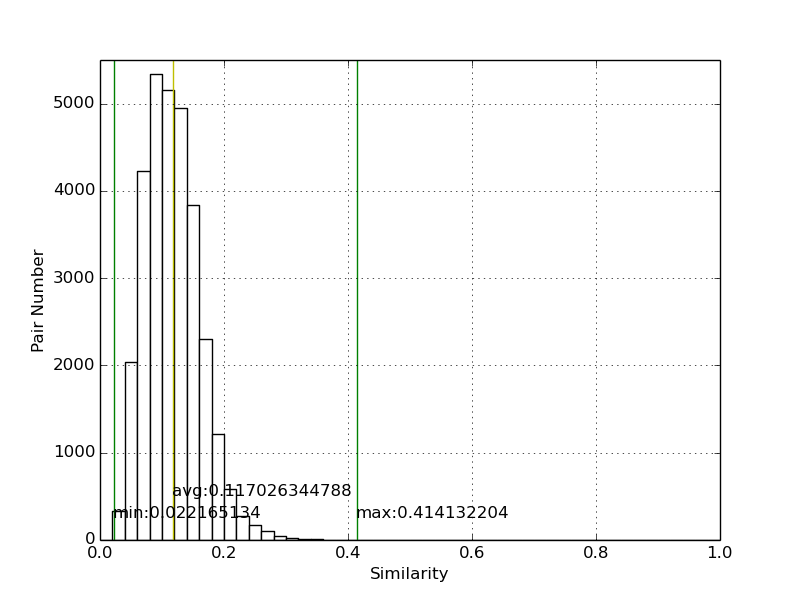
\includegraphics[width=3in]{normalized_similarity_distribution.png}
\end{center}

\begin{center}
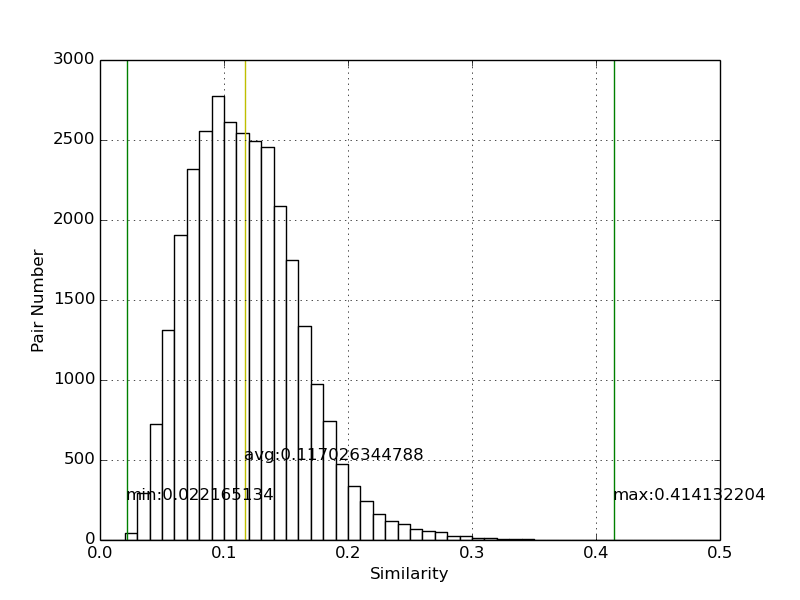
\includegraphics[width=3in]{extended_normalized_similarity_distribution.png}
\end{center}

And the normalized average similarity in category are shown below:

\begin{center}
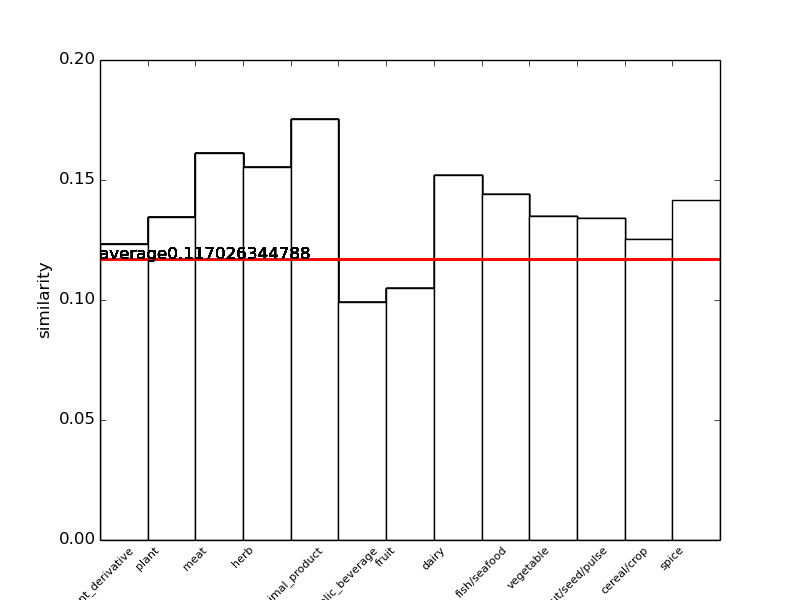
\includegraphics[width=3in]{normalized_similarity_by_category.png}
\end{center}

On the other hand, a common way to compare the similarity among vectors is calculating distance metric. In word2vec, the similarity of the vectors are given by their cosine:
\begin{equation}
\begin{split}
cosine\_similarity(A,B) = \cos(\theta) = \\
\frac{A \cdot B}{\|A\|\|B\|} = \frac{\sum_{i=1}^{n}A_iB_i}{\sqrt{\sum_{i=1}^{n}A_i^2}\sqrt{\sum_{i=1}^{n}B_i^2}}
\end{split}
\end{equation}
Since in vector file, their are negative values, the cosine similarity is bounded between $[-1,1]$. 

In order to obtain a similarity metric that is bounded between [0,1], we need to transform the cosine similarity to angular similarity by:
\begin{equation}
\begin{split}
angular\_similarity(A,B) = \\
1- \frac{\cos^{-1}(cosine\_similarity(A,B))}{\pi}
\end{split}
\end{equation}
By plotting this similarity distribution, we get graph as below:
\begin{center}
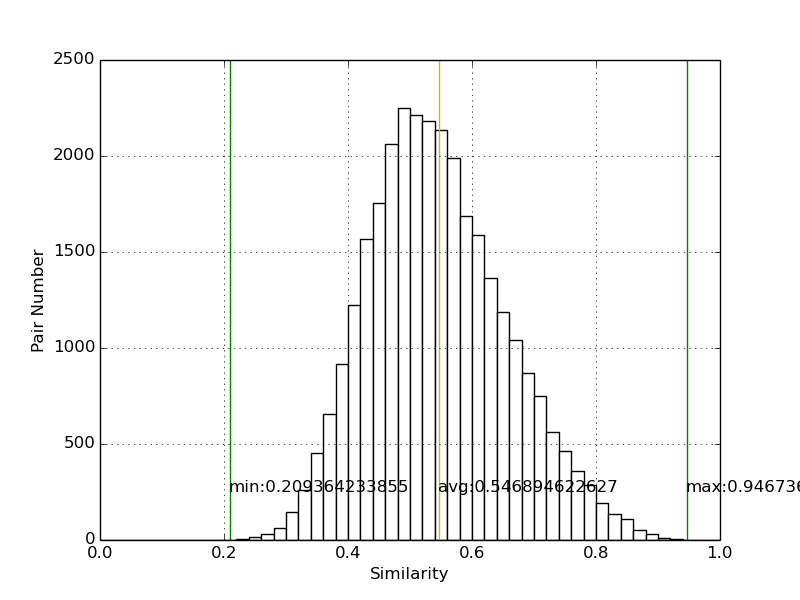
\includegraphics[width=3in]{angular_similarity_distribution.png}
\end{center}

However, the distribution of angular similarity does not have a shape similar to the normalized similarity distribution that we talked above. To explore if these two similarity measures agree to each other, I try to sort both similarity matrix (the angular similarity matrix and the normalized similarity matrix), and compare if they have same ordering of most similar ingredients in each row. 
For example, considering ingredient 'beef', according to the normalized similarity, top 15 most similar ingredients are: celery\_oil, tamarind, kidney\_bean, tomato\_juice, tomato, beef\_broth, green\_bell\_pepper, oregano, onion, roasted\_beef, garlic, black\_bean, cayenne, bay, okra. And according to angular similarity, its top 15 most similar ingredients are: tomato\_juice, beef\_broth, onion, garlic, roasted\_beef, pork'
 'black\_pepper, meat, bean, green\_bell\_pepper, bell\_pepper, tomato'
 'carrot, tamarind, vinegar. The number of common ones are calculated and averaged among all 248 ingredients. And it turns out that these two measures only partially (at best 35%) agree with each other.


\end{multicols}
\end{document}
